\documentclass[titlepage]{article}
\usepackage[utf8]{inputenc}
\usepackage[margin=1in]{geometry}
\usepackage{booktabs}
\usepackage{array}
\usepackage{hyperref}
\usepackage{graphicx}
\usepackage{longtable}
\bibliographystyle{plain}

% TODO: Consider adding a table of contents with \tableofcontents

\title{Implementation and Evaluation of KNN and SVM Classification Configurations, with Instance Reduction Techniques}
\author{Zachary Parent, Sheena Lang, Kacper Poniatowski and Carlos Jiménez}
\date{\today}

\begin{document}

\maketitle

\tableofcontents
\newpage

\section{Introduction}
\label{sec:introduction}

Machine learning classification algorithms play a crucial role in modern data analysis, enabling automated decision-making across diverse domains from medical diagnostics to pattern recognition. This study focuses on evaluating and comparing two fundamental classification algorithms: k-Nearest Neighbors (KNN) and Support Vector Machines (SVM), along with instance reduction techniques to improve their efficiency.

\subsection{Background}

Classification algorithms assign predefined categories to data points based on their features. While many sophisticated classification methods exist, KNN and SVM remain widely used due to their interpretability and strong theoretical foundations. KNN operates by examining the closest training examples to make predictions, while SVM finds optimal hyperplanes to separate classes in feature space.

A key challenge with instance-based methods like KNN is their computational and storage requirements, 
particularly for large datasets. Instance reduction techniques address this limitation by identifying 
and preserving only the most informative training examples, potentially improving both efficiency 
and generalization \cite{knn}.

\subsection{Research Objectives}

This study addresses three primary research questions:

\begin{enumerate}
    \item How do KNN and SVM compare in terms of classification accuracy and computational efficiency across datasets with different characteristics?
    \item What impact do various distance metrics, weighting schemes, and kernel functions have on model performance?
    \item Can instance reduction techniques maintain classification accuracy while significantly reducing storage and computational requirements?
\end{enumerate}

\subsection{Methodology Overview}

We evaluate these questions using two carefully selected datasets:
\begin{itemize}
    \item The Mushroom dataset (8,124 instances) - featuring categorical attributes and balanced classes
    \item The Hepatitis dataset (155 instances) - containing mixed data types and imbalanced classes
\end{itemize}

Our analysis employs rigorous statistical testing to compare model configurations and reduction techniques. We use cross-validation and multiple performance metrics to ensure robust conclusions.

\subsection{Contributions}

The key contributions of this work include:
\begin{itemize}
    \item A comprehensive comparison of KNN and SVM performance across diverse dataset characteristics
    \item Empirical evaluation of three instance reduction techniques (GCNN, ENNTh, and DROP3)
    \item Statistical analysis framework for comparing classification algorithms and reduction methods
    \item Practical guidelines for choosing between KNN and SVM based on dataset properties
\end{itemize}

\subsection{Report Structure}

The remainder of this report is organized as follows:
\begin{itemize}
    \item Section 2 describes the datasets and preprocessing methodology
    \item Section 3 details the implementation of KNN, SVM, and reduction techniques
    \item Section 4 presents experimental results and statistical analysis
    \item Section 5 concludes with key findings and future research directions
\end{itemize}
\section{Data}
\label{sec:data}

\subsection{Dataset}
\label{subsec:dataset}

In this section, we describe the selection criteria that guided our choice of the Mushroom and Hepatitis datasets and analyze their respective characteristics.

\subsubsection{Dataset Selection}
In this project, we aimed to select two datasets that offer substantial variability across different aspects to evaluate the performance of Support Vector Machine (SVM) and k-Nearest Neighbors (KNN) algorithms.
The criteria for dataset selection were centered around having one dataset that is small and another that is large, allowing us to analyze both the efficiency and effectiveness of these models across differing dataset sizes.
A smaller dataset, enables rapid experimentation and comparison of SVM and KNN performance.
Meanwhile, a larger dataset, provides an excellent opportunity to evaluate the benefits of reduction methods in KNN, especially regarding storage efficiency and reduced running time \cite{distance_func_knn}.

Moreover, we wanted to assess the models' ability to handle datasets with different types of attributes.
For this purpose, we wanted to select one dataset with primarily nominal attributes and another with numerical features.
This allows us to evaluate how well each algorithm handles the representation and processing of different data types.
Additionally, class distribution was a critical factor in our selection. By choosing one dataset with a balanced distribution and another with a notable class imbalance, we aim to observe how SVM and KNN, particularly with reduction, perform in scenarios where the data is skewed.
Lastly, we prioritized finding datasets with varying levels of missing data to examine how effectively the algorithms manage incomplete information.

Based on these criteria, we selected the Hepatitis and Mushroom datasets, as they provide the most distinct and complementary combination for our evaluation.

\subsubsection{Dataset Characteristics}

\begin{figure}
    \centering
    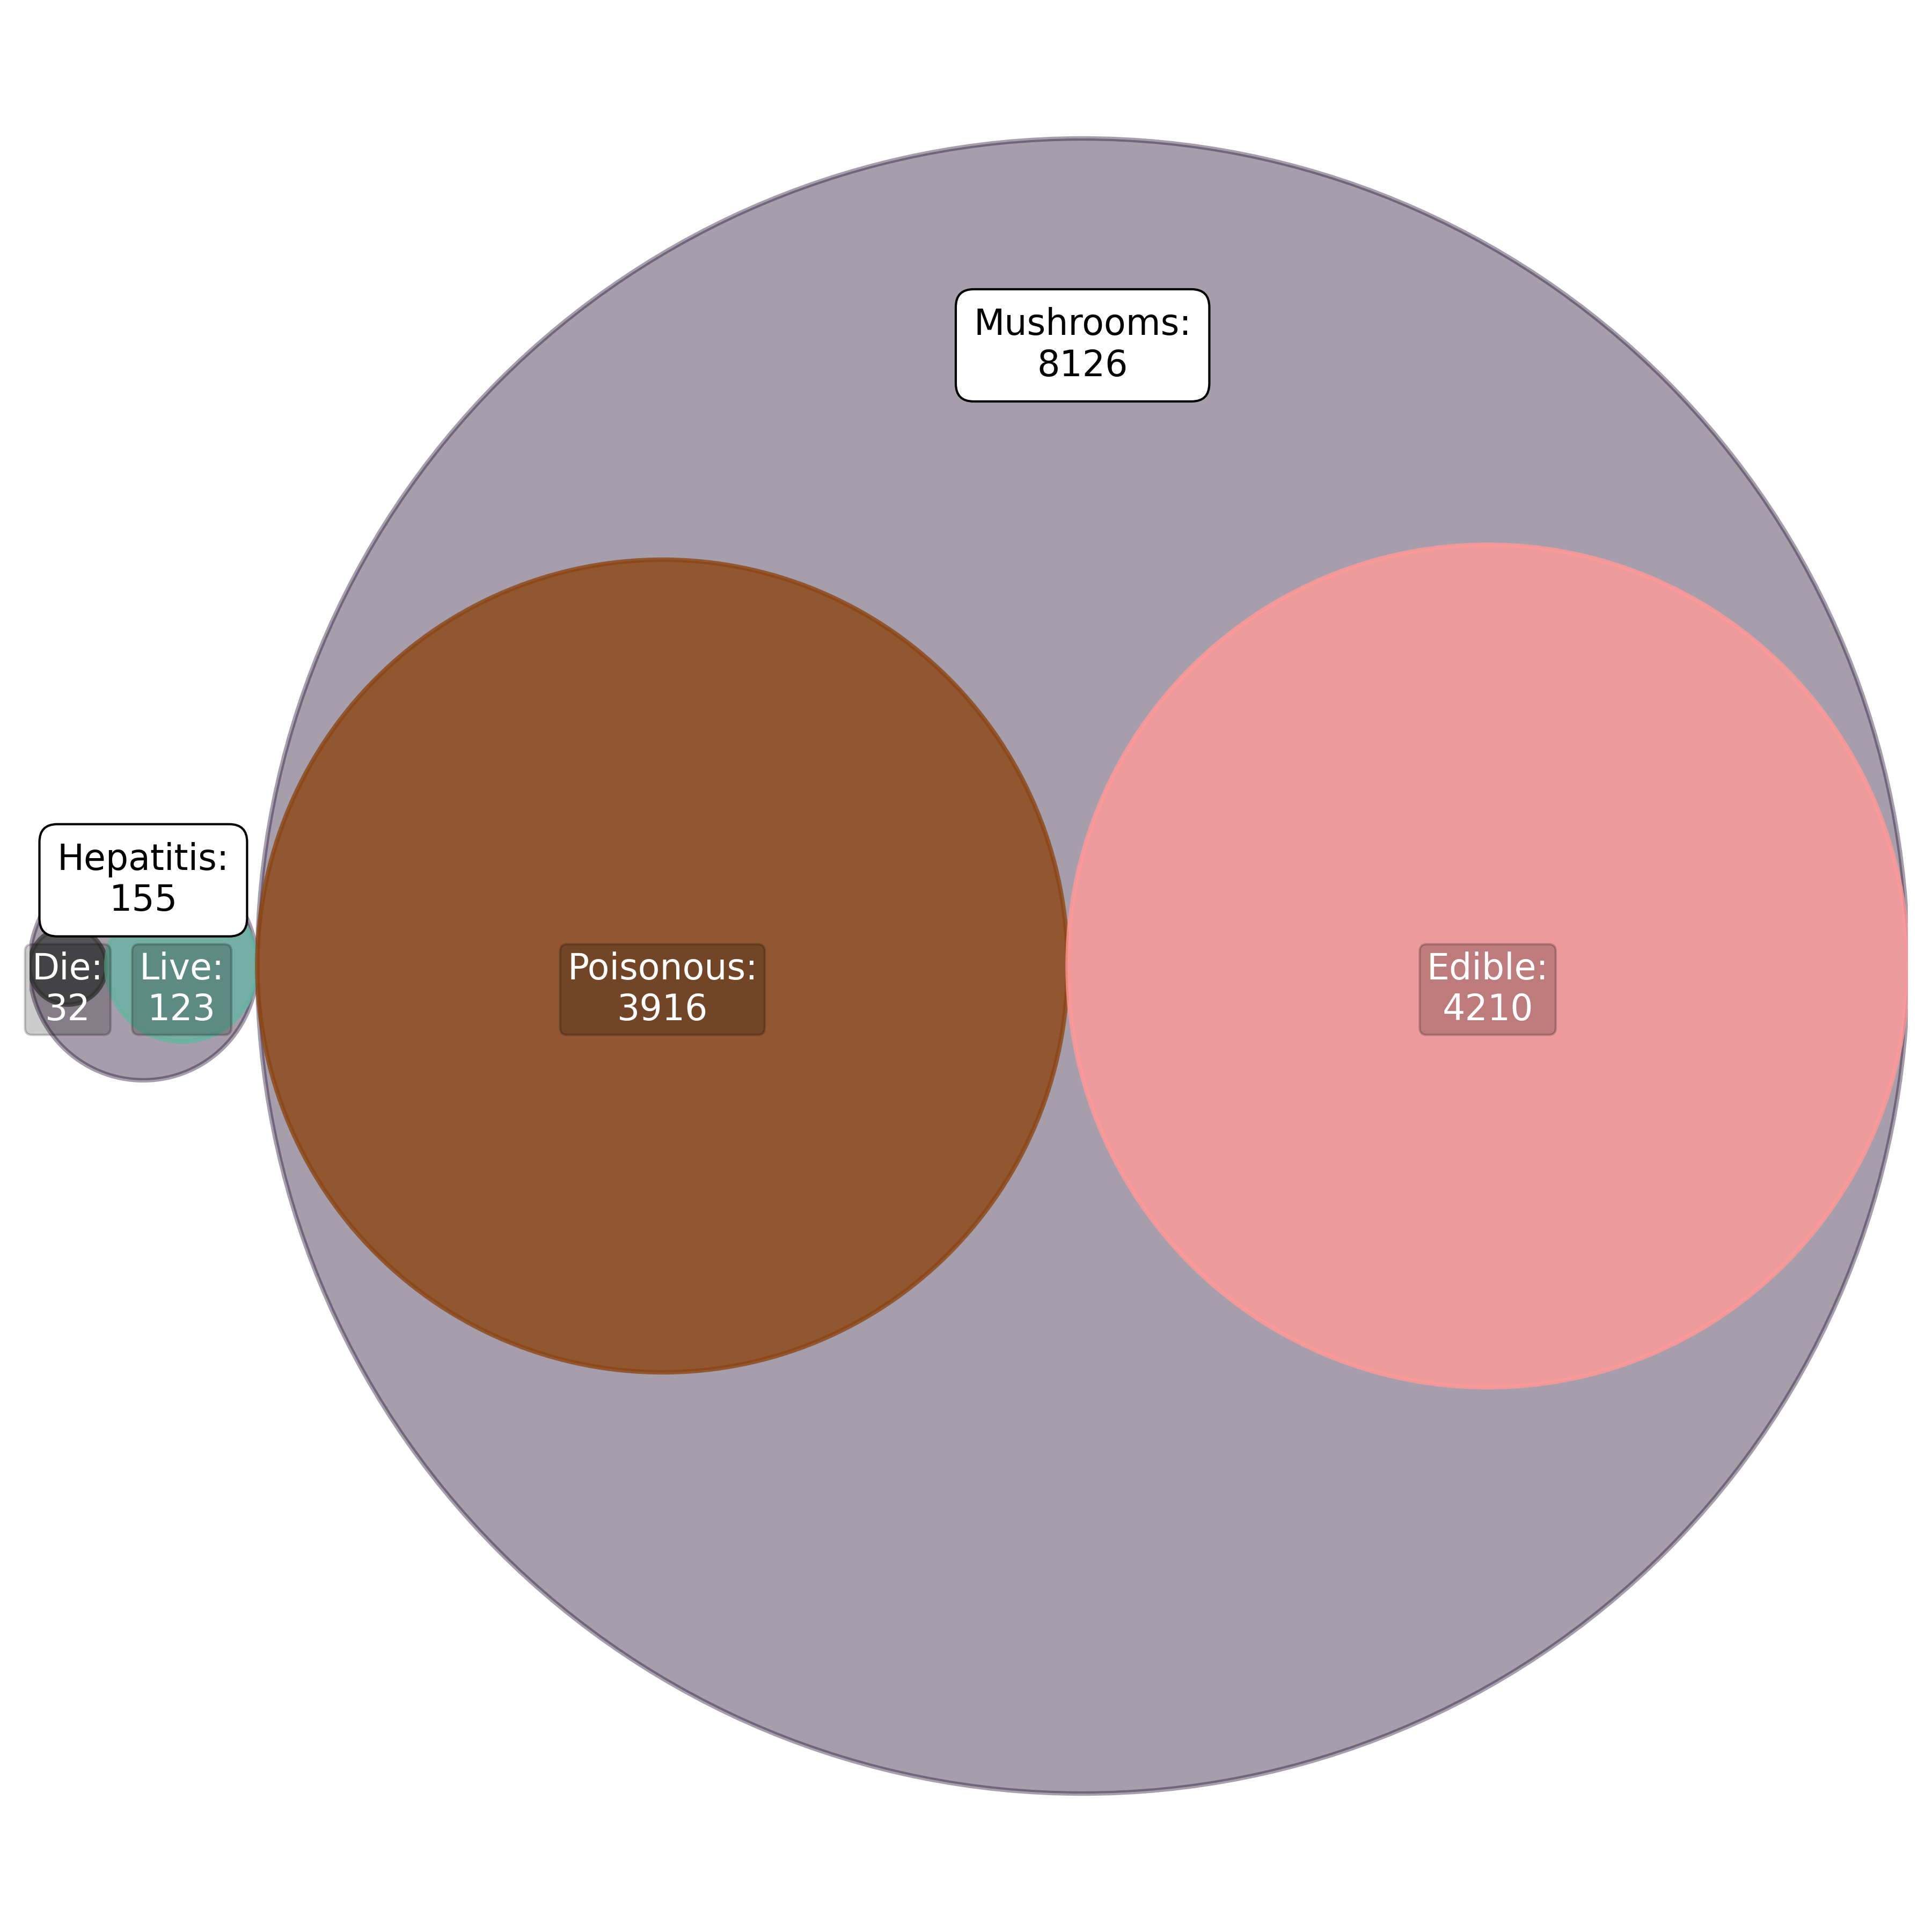
\includegraphics[width=0.5\textwidth]{figures/dataset-partitions.png}
    \caption{Dataset partitions}
    \label{fig:dataset-partitions}
\end{figure}

The Mushroom dataset, with 8,124 instances, is much larger (see \autoref{fig:dataset-partitions}) than the Hepatitis dataset's 155 instances, making it ideal for examining the computational benefits of reduction techniques.
The Mushroom dataset focuses on predicting whether a mushroom is poisonous or edible based on 22 nominal attributes, such as cap shape and color, whereas the Hepatitis dataset aims to predict whether a hepatitis patient will live or die, using a mix of both nominal and numeric features like age and liver size.
This allows for a comparison of model handling for fully categorical data versus mixed data types.

\begin{figure}
    \centering
    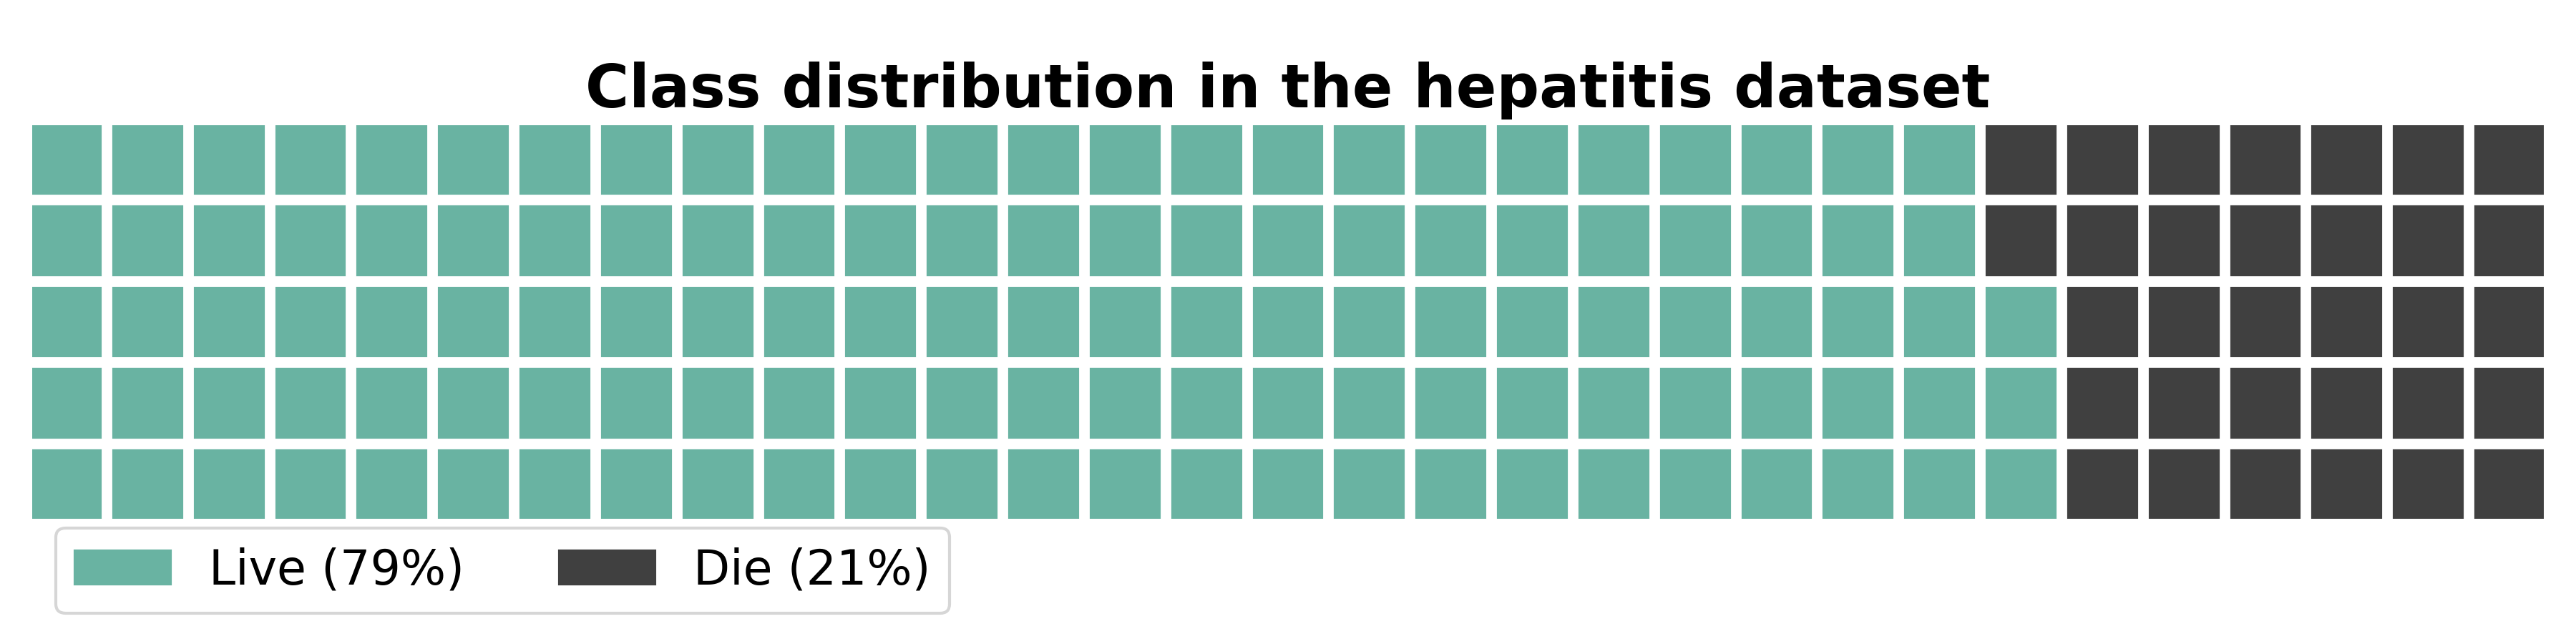
\includegraphics[width=0.45\textwidth]{figures/hepatitis-class-distribution.png}
    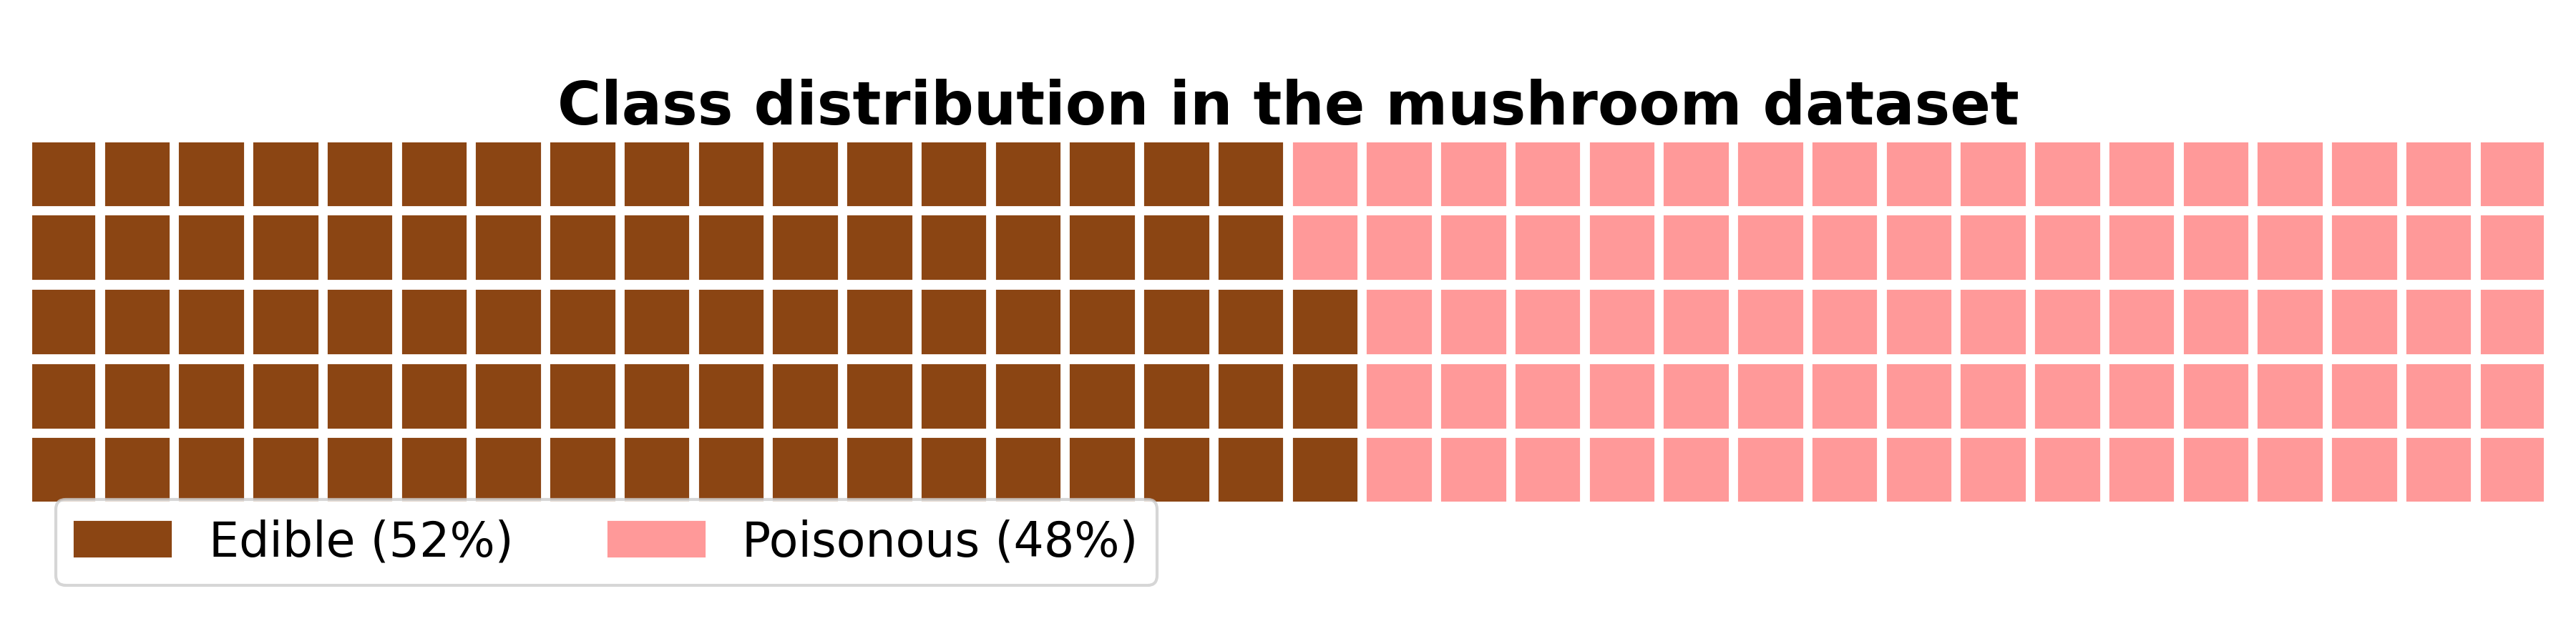
\includegraphics[width=0.45\textwidth]{figures/mushroom-class-distribution.png}
    \caption{Class distributions}
    \label{fig:class-distributions}
\end{figure}

Class distribution is another key distinction.
The Mushroom dataset is nearly balanced, with only a 1.8\% class deviation, while the Hepatitis dataset has a 29.35\% class deviation, with 79.35\% of instances in the majority class (see \autoref{fig:class-distributions}), making it ideal for testing each model's robustness to imbalanced data.
Missing data is also more prevalent in the Mushroom dataset (48.2\%) compared to Hepatitis (20.01\%), providing insights into each model’s ability to handle incomplete data.
\subsection{Data Preprocessing}
\label{subsec:preprocessing}

This section outlines the preprocessing steps applied to the Hepatitis and Mushroom datasets.

\subsubsection{Dealing with Different Ranges and different types}
To manage the varying types and ranges of attributes in our datasets, we implemented specific preprocessing techniques.
For the nominal attributes in both the Mushroom and Hepatitis datasets, we used label encoding.
This technique converts categorical values into numerical labels, enabling the algorithms to interpret the data correctly.
While we considered one-hot encoding to avoid implying any ordinal relationship among categories, we opted for label encoding due to its simplicity and reduced dimensionality, as one-hot encoding would significantly increase dimensions and lead to a sparse space, making accurate predictions more challenging, particularly for KNN with the Mushroom dataset's numerous nominal features.

For the numerical attributes in the Hepatitis dataset, we applied min-max scaling to rescale the data to a fixed range of [0, 1]. This normalization is crucial for distance-based algorithms like KNN and SVM, ensuring all features contribute equally to model performance.
We evaluated other scaling methods, such as standardization, but chose min-max scaling for its effectiveness in maintaining the original data distribution \cite{data_cleaning}.

\subsubsection{Dealing with Missing Values}
Addressing missing values is a critical step in preparing our datasets for analysis, as they can significantly impact model performance.
In the case of the nominal attributes in both the Mushroom and Hepatitis datasets, we opted to impute missing values with the majority class.
This method is straightforward and effective for maintaining dataset integrity.
However, it can also introduce bias, particularly in the Hepatitis dataset, where the majority class represents 79.35\% of instances.
Relying on this method may lead to a situation where the imputed values disproportionately favor the majority class, thereby affecting the overall distribution
and potentially skewing the results \cite{data_cleaning}.

For the numerical attributes in the Hepatitis dataset, we used the mean of the available data to fill in missing values.
This approach preserves the overall data distribution and is easy to implement, but it is not without its drawbacks.
The mean can be heavily influenced by outliers, which might distort the data and lead to less accurate predictions.
This is especially important in medical datasets, where extreme values may carry significant meaning.

We also considered employing K-Nearest Neighbors (KNN) for imputing missing values, as it could provide a more nuanced approach by considering the nearest data points for each instance.
However, we ultimately decided against this option to avoid introducing bias into our evaluation.
Since KNN is one of the algorithms we are testing, using it for imputation could influence its performance and lead to skewed results.
Therefore, we chose the more straightforward methods of majority class imputation for nominal values and mean imputation for numerical values, allowing for a clearer assessment of the models’ effectiveness without confounding factors.




\section{Methods}
\label{sec:methods}

This section describes the methodology used in the study. It should include details about data collection, experimental design, and analytical techniques.

\subsection{k-Nearest Neighbors (kNN)}
\label{subsec:methods-knn}

This section describes the k-Nearest Neighbors (kNN) algorithm and its implementation in our study.

% TODO: Provide a brief overview of the kNN algorithm
% TODO: Explain the choice of k value and any cross-validation used
% TODO: Describe the distance metric used (e.g., Euclidean, Manhattan)
% TODO: Discuss any feature scaling or normalization applied specifically for kNN

\subsubsection{Algorithm Overview}
% TODO: Explain how kNN works and its advantages/disadvantages

\subsubsection{Implementation Details}
% TODO: Describe the specific implementation, including any libraries or tools used

\subsubsection{Parameter Tuning}
% TODO: Explain how parameters were chosen and optimized

% Add more content here as needed


\subsection{Instance Reduction Algorithms}
\label{subsec:methods-reduction}

A significant challenge in applying kNN to large datasets is the computational cost 
associated with searching the entire training set. Additionally, noisy or irrelevant 
data can negatively impact the model's performance. 
To overcome these issues, we employ instance reduction techniques. 
These techniques aim to identify and select a smaller, more representative subset of
the training data, leading to faster prediction times and improved accuracy \cite{Wilson2000}.\\

A variety of rule-based techniques have been proposed in the literature to 
address the challenges associated with large and noisy datasets. 
These techniques aim to identify patterns and relationships within the data to select 
a subset of informative instances.

\subsubsection{Condensed Nearest Neighbour Rule}
Condensed nearest neighbor rules (CNN) are a family of algorithms that aim to identify 
a minimal subset of the training data that can represent the entire dataset without 
significant loss of information. One prominent example is the \textbf{Generalized Condensed 
Nearest Neighbor} (GCNN) algorithm.
% GCNN iteratively selects instances that are misclassified by the current reduced set, 
% adding them to the reduced set until no further improvement is possible. 
% This technique effectively reduces the dataset size while preserving essential 
% information for accurate classification.

GCNN \cite{hart1968condensed} is an iterative algorithm that starts with a small subset of 
the training data and incrementally adds instances that are misclassified by the current KNN model. 
This process continues until no further instances are misclassified. GCNN aims to identify a minimal 
consistent subset, a subset of the original data that correctly classifies all of the original 
instances using the 1-NN rule.

More formally, let $X = \{x_1, x_2, ..., x_n\}$ be the set of training instances and $Y = \{y_1, y_2, ..., y_n\}$ be 
the corresponding class labels. GCNN can be described as follows:

\begin{enumerate}
    \item \textbf{Initialization:} Select a random instance $x_i$ from $X$ and add it to the condensed set $C$.
    \item \textbf{Iteration:} For each instance $x_j \in X \setminus C$:
    \begin{itemize}
        \item Train a 1-NN classifier on $C$.
        \item If $kNN(x_j) \neq y_j$, then add $x_j$ to $C$.
    \end{itemize}
    \item \textbf{Termination:} Repeat step 2 until no new instances are added to $C$.
\end{enumerate}

GCNN's effectiveness lies in its ability to capture the decision boundaries between classes using a reduced 
set of instances. However, its performance can be sensitive to the initial instance selection and the order 
in which instances are processed.



\subsubsection{Edited Nearest Neighbour Rule}
Edited nearest neighbor rules, on the other hand, focus on removing noisy or outlier 
instances from the training data. 

The \textbf{Edited Nearest Neighbor Estimating Class Probabilistic and Threshold (ENNTh)} is a noise-removal technique that builds upon the Edited Nearest Neighbor (ENN) algorithm \cite{wilson2000reduction}. ENN aims to improve the generalization ability of KNN by removing instances that are likely to be noise or outliers. ENNTh refines this process by incorporating a threshold, $\tau$, to control the degree of noise removal. [CITE]

ENN traditionally removes an instance if its class label differs from the majority class among its $k$ nearest neighbors. ENNTh introduces a more flexible approach by estimating the class probability of an instance based on its $k$ nearest neighbors. Let $N_k(x_i)$ denote the set of $k$ nearest neighbors of $x_i$. The class probability of $x_i$ is estimated as:

\begin{equation}
P(y_i | x_i) = \frac{|\{x_j \in N_k(x_i) : y_j = y_i\}|}{k}
\end{equation}

An instance $x_i$ is removed only if $P(y_i | x_i) < \tau$. This thresholding mechanism allows for a more nuanced approach to noise removal, where instances with a higher probability of belonging to their assigned class are retained, even if they are not in the majority class among their neighbors.

By adjusting the threshold $\tau$, ENNTh can control the trade-off between noise removal and the preservation of potentially useful instances. A higher threshold leads to more aggressive noise removal, while a lower threshold retains more instances. [CITE]


% \subsubsection{Hybrid Reduction Techniques}
% Hybrid reduction techniques combine the strengths of both condensed and edited approaches
% to achieve more robust and efficient reduction. The \textbf{Drop2} algorithm is a notable example
% of a hybrid technique. It first applies a condensed nearest neighbor rule to identify a
% core set of instances. Then, it uses an edited nearest neighbor rule to further refine
% the reduced set by removing noisy or redundant instances.
% This two-step process results in a compact and informative dataset.

\subsubsection{Hybrid Reduction Techniques}

Hybrid reduction techniques combine the strengths of both condensed and edited approaches to 
achieve more robust and efficient reduction. The \textbf{DROP3} algorithm \cite{wilson2000reduction} 
is a notable example of a hybrid technique. Unlike DROP2, which uses CNN first and then ENN, DROP3 reverses this order. 
It first applies an edited nearest neighbor rule (ENN) to remove noisy or borderline instances, creating a cleaner dataset.
Then, it employs a decremental reduction procedure inspired by condensed nearest neighbor to iteratively remove redundant
instances that do not affect the classification accuracy of their neighbors. This process results in a significantly 
reduced dataset while aiming to preserve classification accuracy.

DROP3 \cite{wilson2000reduction} is a hybrid instance reduction technique that combines the strengths of ENN and Condensed Nearest Neighbor (CNN). It aims to achieve a more substantial reduction in the dataset size while maintaining or improving classification accuracy.\\

DROP3 operates in two main stages:

\begin{enumerate}
    \item \textbf{Noise Removal:} In the first stage, DROP3 applies ENN to the training set $(X, Y)$ to eliminate noisy instances. This step helps to improve the quality of the data and prepare it for further reduction. 
    \item \textbf{Iterative Reduction:} The second stage involves an iterative process where each remaining instance is evaluated for potential removal. An instance is removed if its removal does not adversely affect the classification accuracy of its neighbors.  More specifically, for each instance $x_i$, DROP3 trains a KNN classifier on the dataset excluding $x_i$, $(X' \setminus \{x_i\}, Y' \setminus \{y_i\})$. If all instances in $N_k(x_i)$ are correctly classified by this KNN classifier, then $x_i$ is deemed redundant and removed.
\end{enumerate}

This iterative process continues until no further instances can be removed without affecting the classification accuracy of their neighbors. DROP3 effectively identifies and removes redundant instances that do not contribute significantly to the classification performance. By combining noise removal with iterative reduction, DROP3 achieves a more aggressive reduction in the dataset size compared to ENN or CNN alone.


\subsection{Support Vector Machines (SVM)}
\label{subsec:methods-svm}

This section describes the Support Vector Machines (SVM) algorithm and its implementation in our study.

\subsubsection{Algorithm Overview}

Support Vector Machines (SVM) is a powerful supervised learning algorithm used for classification and
regression tasks. The primary objective of SVM is to find the optimal hyperplane that separates different classes
in the feature space while maximizing the margin between the classes\cite{burges1998svmTutorial}.

The key principles of SVM include:

\begin{itemize}
    \item Margin Maximization: SVM aims to find the hyperplane that maximizes the margin between classes, which enhances the model's generalization capability.
    \item Support Vectors: The data points closest to the decision boundary, known as support vectors, play a crucial role in defining the optimal hyperplane.
    \item Kernel Trick: SVM can handle non-linearly separable data by mapping the input space to a higher-dimensional feature space using kernel functions.
\end{itemize}

Advantages of SVM include:
\begin{itemize}
    \item Effectiveness in high-dimensional spaces
    \item Versatility through different kernel functions
    \item Faster consultation times than KNN, thanks to training step
\end{itemize}

Disadvantages of SVM include:
\begin{itemize}
    \item Sensitivity to the choice of kernel function and hyperparameters
    \item Computational complexity for large datasets
\end{itemize}
\subsubsection{Implementation Details}

Unlike for KNN (see \autoref{subsec:methods-knn} on K-Nearest Neighbors), we did not implement the SVM algorithm ourselves.
Instead, we used the prebuilt implementations from the \texttt{sklearn} library
\footnote{Scikit-learn's \texttt{svm} module documentation can be found at \url{https://scikit-learn.org/1.5/modules/svm.html}}.
Scikit-learn's \texttt{svm} module includes several different implementations of SVM:

\begin{itemize}
    \item \texttt{SVC}: Support Vector Classification, the most commonly used implementation for classification tasks
    \item \texttt{NuSVC}: Support Vector Classification with Nu-SVC, similar to \texttt{SVC} but with a different formulation of the optimization problem 
    \item \texttt{LinearSVC}: Linear Support Vector Classification, a specific variant of \texttt{SVC} that uses a linear kernel
    \item \texttt{SVR}: Support Vector Regression, a variant of SVM for regression tasks
\end{itemize}

For our study, we decided to use \texttt{SVC} as it is the most commonly used implementation
for classification tasks, allowed for the kernel trick (unlike \texttt{LinearSVC}), and met our needs.

\subsubsection{Kernel Selection}

In our study, we explored multiple kernel functions to capture different types of relationships in the data. The kernels used include:

\begin{itemize}
    \item Linear: $K(x_i, x_j) = x_i^T x_j$
    \item Polynomial: $K(x_i, x_j) = (\gamma x_i^T x_j + r)^d$
    \item Radial Basis Function (RBF): $K(x_i, x_j) = \exp(-\gamma ||x_i - x_j||^2)$
    \item Sigmoid: $K(x_i, x_j) = \tanh(\gamma x_i^T x_j + r)$
\end{itemize}

Where $x_i$ and $x_j$ are feature vectors, $\gamma$ is a kernel coefficient, $r$ is a constant term, and $d$ is the degree of the polynomial kernel.

\subsubsection{Hyperparameter Tuning}

The following hyperparameters were tuned in our SVM implementation:

\begin{itemize}
    \item C: The regularization parameter, which controls the trade-off between achieving a low training error and a low testing error. We explored values [1, 3, 5, 7].
    \item Kernel: We tested different kernel types including "linear", "poly", "rbf", and "sigmoid".
\end{itemize}

\subsubsection{Implementation Steps}

The SVM classification process in our study followed these steps:

\begin{enumerate}
    \item Data Preparation (see \autoref{sec:data} on Data).
    \item Model Configuration: SVM models were created with different combinations of C values and kernel types.
    \item Cross-validation: For each configuration, the model was trained and evaluated using cross-validation across 10 predefined folds.
    \item Performance Evaluation: Various metrics including accuracy, F1 score, and confusion matrix elements (TP, TN, FP, FN) were computed.
    \item Time Measurement: Training and testing times were recorded for each configuration.
    \item Results Compilation: The results for each configuration were saved in CSV files for further analysis.
\end{enumerate}

\subsubsection{Multi-class Classification}

While simple SVMs are binary classifiers, they can be extended to multi-class classification through various strategies.
In our case, however, both the datasets included only two classes, so we did not need to use these strategies.

\subsubsection{Performance Metrics}

The performance of the SVM models was evaluated using the following metrics:

\begin{itemize}
    \item Accuracy: The proportion of correct predictions among the total number of cases examined.
    \item F1 Score: The harmonic mean of precision and recall, providing a balanced measure of the model's performance.
    \item Confusion Matrix: Including True Positives (TP), True Negatives (TN), False Positives (FP), and False Negatives (FN).
    \item Training Time: The time taken to train the model.
    \item Testing Time: The time taken to make predictions on the test set.
\end{itemize}

The F1 score was used as our primary metric for evaluating the performance of the SVM models,
since it balances the trade-off between precision and recall, and does not report overly favorable results when the dataset is imbalanced.



% Add more content here as needed

\section{Results and Analysis}
\label{sec:results-and-analysis}

\subsection{Results}
\label{subsec:results}

Here, present the findings of the study. Include relevant data, statistics, and any figures or tables that help illustrate the results.

% TODO: Present main findings clearly and concisely
% TODO: Include relevant statistical analyses
% TODO: Add figures and tables to illustrate key results
% TODO: Ensure all figures and tables are properly labeled and referenced in the text
% TODO: Organize results in a logical order, possibly mirroring the order of the methods

% Add more content here as needed
\begin{table}
\centering
\caption{Results from KNN models for the mushroom dataset}
\begin{tabular}{lrrlllrr}
\toprule
 &  & k & distance func & voting func & weighting func & accuracy & f1 \\
\midrule
0 & 1 & 7 & ManhattanDistance & ShepardsWorkVote & EqualWeighting & 0.951 & 0.952 \\
1 & 2 & 5 & ManhattanDistance & ShepardsWorkVote & EqualWeighting & 0.951 & 0.952 \\
2 & 3 & 3 & ManhattanDistance & ShepardsWorkVote & EqualWeighting & 0.951 & 0.952 \\
3 & 4 & 1 & ManhattanDistance & MajorityClassVote & EqualWeighting & 0.950 & 0.951 \\
4 & 5 & 1 & ManhattanDistance & InverseDistanceWeightedVote & EqualWeighting & 0.950 & 0.951 \\
5 & 6 & 1 & ManhattanDistance & ShepardsWorkVote & EqualWeighting & 0.950 & 0.951 \\
6 & 7 & 5 & ManhattanDistance & InverseDistanceWeightedVote & EqualWeighting & 0.933 & 0.933 \\
7 & 8 & 7 & ManhattanDistance & InverseDistanceWeightedVote & EqualWeighting & 0.930 & 0.929 \\
8 & 9 & 3 & ManhattanDistance & InverseDistanceWeightedVote & EqualWeighting & 0.928 & 0.929 \\
9 & 10 & 3 & ManhattanDistance & MajorityClassVote & EqualWeighting & 0.926 & 0.927 \\
\bottomrule
\end{tabular}
\end{table}

.\begin{table}
\centering
\caption{Results From Knn Models For The Hepatitis Dataset}
\label{tab:knn_results_hepatitis}
\begin{tabular}{rlrrr}
\toprule
 & Model Label & Mean F1 & Mean Train Time (s) & Mean Test Time (s) \\
\midrule
1 & k1ChebShpEq & 0.972618 & 0.000084 & 0.006925 \\
2 & k1ChebMajEq & 0.972618 & 0.000085 & 0.006949 \\
3 & k1ChebDisEq & 0.972618 & 0.000084 & 0.006896 \\
4 & k5EucShpEq & 0.969271 & 0.000084 & 0.009300 \\
5 & k7EucShpEq & 0.969271 & 0.000083 & 0.009293 \\
6 & k3ManShpEq & 0.969231 & 0.000083 & 0.007033 \\
7 & k1ManMajEq & 0.969231 & 0.000120 & 0.007153 \\
8 & k1EucShpRlf & 0.969231 & 0.000084 & 0.009349 \\
9 & k1ManShpEq & 0.969231 & 0.000083 & 0.006982 \\
10 & k1EucMajEq & 0.969231 & 0.000086 & 0.009228 \\
\bottomrule
\end{tabular}
\end{table}

\begin{table}
\centering
\caption{Results from SVM models for the mushroom dataset}
\begin{tabular}{lrrlrr}
\toprule
 &  & C & kernel type & accuracy & f1 \\
\midrule
0 & 1 & 1 & poly & 0.928 & 0.928 \\
1 & 2 & 7 & rbf & 0.926 & 0.926 \\
2 & 3 & 5 & rbf & 0.925 & 0.925 \\
3 & 4 & 3 & rbf & 0.924 & 0.924 \\
4 & 5 & 7 & poly & 0.920 & 0.920 \\
5 & 6 & 5 & poly & 0.916 & 0.916 \\
6 & 7 & 3 & poly & 0.916 & 0.915 \\
7 & 8 & 3 & linear & 0.914 & 0.912 \\
8 & 9 & 1 & linear & 0.911 & 0.910 \\
9 & 10 & 1 & rbf & 0.906 & 0.902 \\
\bottomrule
\end{tabular}
\end{table}

\begin{table}
\centering
\caption{Results From Svm Models For The Hepatitis Dataset}
\label{tab:svm_results_hepatitis}
\begin{tabular}{rrlrrr}
\toprule
 & C & kernel type & mean f1 & mean train time & mean test time \\
\midrule
1 & 7 & rbf & 0.975 & 0.001 & 0.000 \\
2 & 5 & rbf & 0.971 & 0.001 & 0.000 \\
3 & 3 & poly & 0.970 & 0.001 & 0.000 \\
4 & 1 & poly & 0.970 & 0.001 & 0.000 \\
5 & 3 & rbf & 0.969 & 0.001 & 0.000 \\
6 & 5 & poly & 0.969 & 0.001 & 0.000 \\
7 & 7 & poly & 0.969 & 0.001 & 0.000 \\
8 & 1 & rbf & 0.942 & 0.001 & 0.000 \\
9 & 3 & linear & 0.929 & 0.001 & 0.000 \\
10 & 1 & linear & 0.927 & 0.001 & 0.000 \\
\bottomrule
\end{tabular}
\end{table}


\subsection{Discussion}
\label{sec:discussion}

In this section, interpret the results, discuss their implications, and relate them back to the research question or hypothesis. Address any limitations of the study and suggest areas for future research.

% TODO: Interpret the results in the context of the research question/hypothesis
% TODO: Compare findings with existing literature
% TODO: Discuss the implications of the results
% TODO: Address any unexpected findings
% TODO: Acknowledge limitations of the study
% TODO: Suggest directions for future research

\subsubsection{k-Nearest Neighbors (kNN) Analysis}
\label{subsubsec:discussion-knn}

This section interprets the results of the kNN algorithm, discussing its performance and implications.

The kNN algorithm was evaluated using several performance metrics, including accuracy, precision, and recall.

% TODO: Summarize the performance metrics of kNN (e.g., accuracy, precision, recall)




\paragraph{Impact of Different k Values}
% The choice of the parameter \( k \) significantly impacts the performance of the kNN algorithm.
% Figure \ref{fig:k-values} illustrates how accuracy varies with different values of \( k \).
% It was observed that the optimal value of \( k \) was 5, beyond which the performance started to degrade.

% \begin{figure}[h]
%     \centering
%     %\includegraphics[width=0.8\textwidth]{path/to/knn-k-values-plot.png}
%     \caption{Impact of different \( k \) values on kNN performance}
%     \label{fig:k-values}
% \end{figure}

\paragraph{Unexpected Findings and Limitations}
One unexpected finding was that the kNN algorithm performed poorly on imbalanced datasets.
This limitation suggests that further preprocessing, such as oversampling or undersampling,
might be necessary to improve performance.

% Add more content here as needed
% TODO: Compare kNN results with other methods used in the study
% TODO: Discuss the impact of different k values on the results
% TODO: Address any unexpected findings or limitations specific to kNN

% Add more content here as needed

\subsubsection{Dimensionality Reduction Analysis}
\label{subsubsec:discussion-reduction}

This section examines the impact of three reduction techniques—GGCN, ENNTH, and Drop3—on the performance, training time, testing time, and storage requirements of both the KNN and SVM algorithms.

For KNN applied to the Hepatitis dataset, applying no redcution yields a high F1 score of 0.9483, with moderate storage requirements of 139.5 units and a testing time of 0.0747 seconds. 
The GGCN reduction technique slightly lowers the F1 score to 0.9354 but significantly improves testing time to 0.0545 seconds and reduces storage to 103.2 units. 
GGCN achieves this by selectively condensing the dataset, retaining instances that best represent the overall data structure and class boundaries. 
By removing redundant points that do not impact classification accuracy, it effectively reduces storage requirements and enhances processing speed without sacrificing much performance.

The F1 score for ENNTH is the same as applying no reduction, and achieves the fastest training time of 0.00042 seconds, but results in almost no reduction in storage since its approach primarily focuses on removing noisy data points at the boundaries. 
Given the relatively low noise in the Hepatitis dataset, ENNTH performs similarly to applying not reduction in terms of storage efficiency. 
Conversely, Drop3 reduces storage to 110.9 units but leads to a more significant drop in the F1 score to 0.9157. 
This reduction in performance can be attributed to Drop3's aggressive removal of instances based on noise and redundancy filtering, which can inadvertently discard valuable data points and degrade predictive accuracy when the dataset is sparse.

When analyzing the Mushroom dataset with KNN, all techniques achieve a perfect F1 score of 1.0, indicating no loss in predictive accuracy. 
GGCN stands out by significantly reducing storage from 7311.6 units to 3519.8 units while also decreasing testing time from 72.78 seconds to 33.70 seconds. 
This effectiveness arises from GGCN’s ability to eliminate redundancy while retaining essential data points, making it particularly advantageous for large datasets. 

ENNTH and Drop3 retain the same storage requirement as the control, both at 7311.6 units, with only slight improvements in training and testing time. 
ENNTH preserves the perfect F1 score by focusing on noise removal, which is less impactful in this dataset due to its inherent cleanliness. 
Similarly, Drop3 achieves a perfect F1 score, as its filtering approach does not affect the well-structured Mushroom dataset.

\begin{figure}
    \centering
    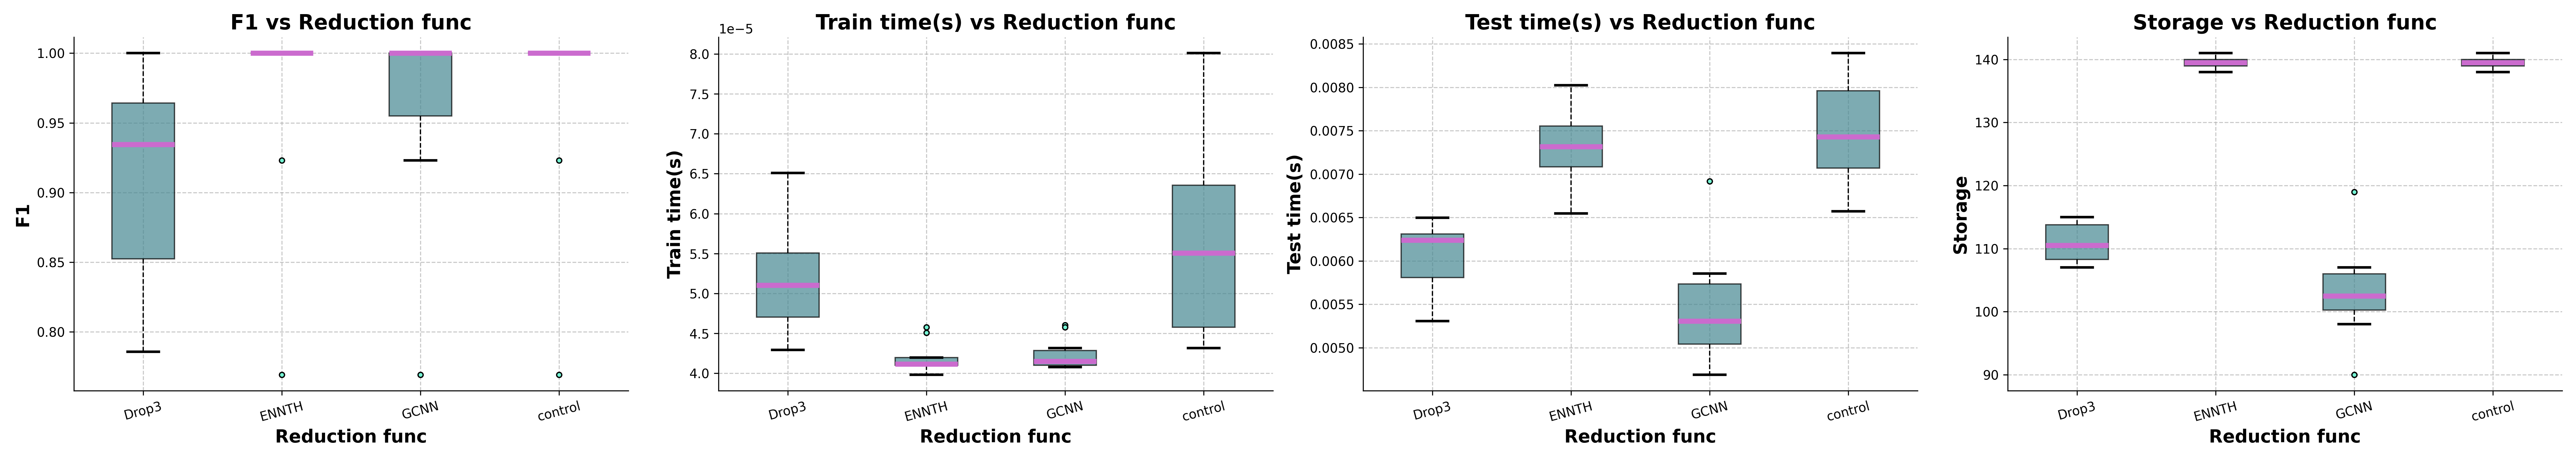
\includegraphics[width=0.45\textwidth]{figures/work2/reports/figures/KNN_reduction_effects_hepatitis.png}
    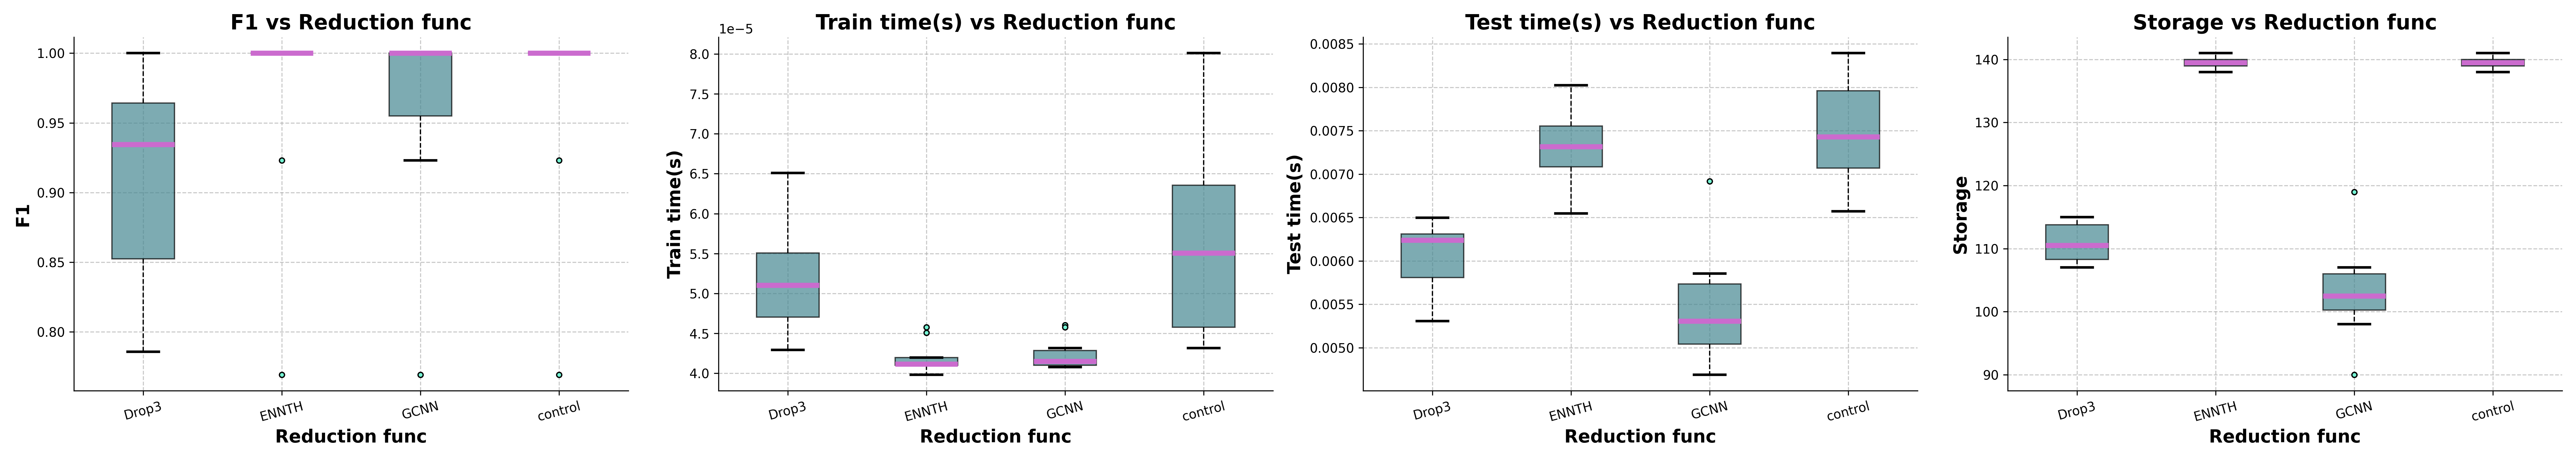
\includegraphics[width=0.45\textwidth]{figures/work2/reports/figures/KNN_reduction_effects_hepatitis.png}
    \caption{Class distributions}
    \label{fig:class-distributions}
\end{figure}

In the context of the Hepatitis dataset using SVM, using no reduction method produces a high F1 score of 0.9719, requiring moderate storage of 139.5 units and a testing time of 0.0037 seconds.
The GGCN technique yields a slightly lower F1 score of 0.9597, but it reduces storage to 103.2 units while maintaining a similar testing time of 0.0037 seconds.

ENNTH maintains the original F1 score of 0.9719 and achieves a testing time of 0.0033 seconds, but it results in almost no storage reduction, as its approach primarily focuses on eliminating noisy boundary points. 
The relatively low noise in the Hepatitis dataset means ENNTH performs comparably to the control in terms of storage usage.
On the other hand, Drop3 reduces storage to 110.9 units but results in a substantial drop in F1 score to 0.9291, reflecting its aggressive filtering approach, which can lead to the loss of critical instances and, consequently, a decline in predictive performance.

For SVM applied to the Mushroom dataset, all methods, yield a perfect F1 score of 1.0, ensuring no predictive accuracy is sacrificed. 
GGCN proves especially effective by reducing storage from 7311.6 units to 3519.8 units and decreasing testing time from 0.0421 seconds to 0.0337 seconds.

ENNTH and Drop3 maintain the same storage requirements as the control, both at 7311.6 units, with minor improvements in training and testing time.
ENNTH’s focus on noise removal contributes to its sustained perfect F1 score, while Drop3’s method similarly does not impact storage significantly in this densely populated dataset.

\begin{figure}
    \centering
    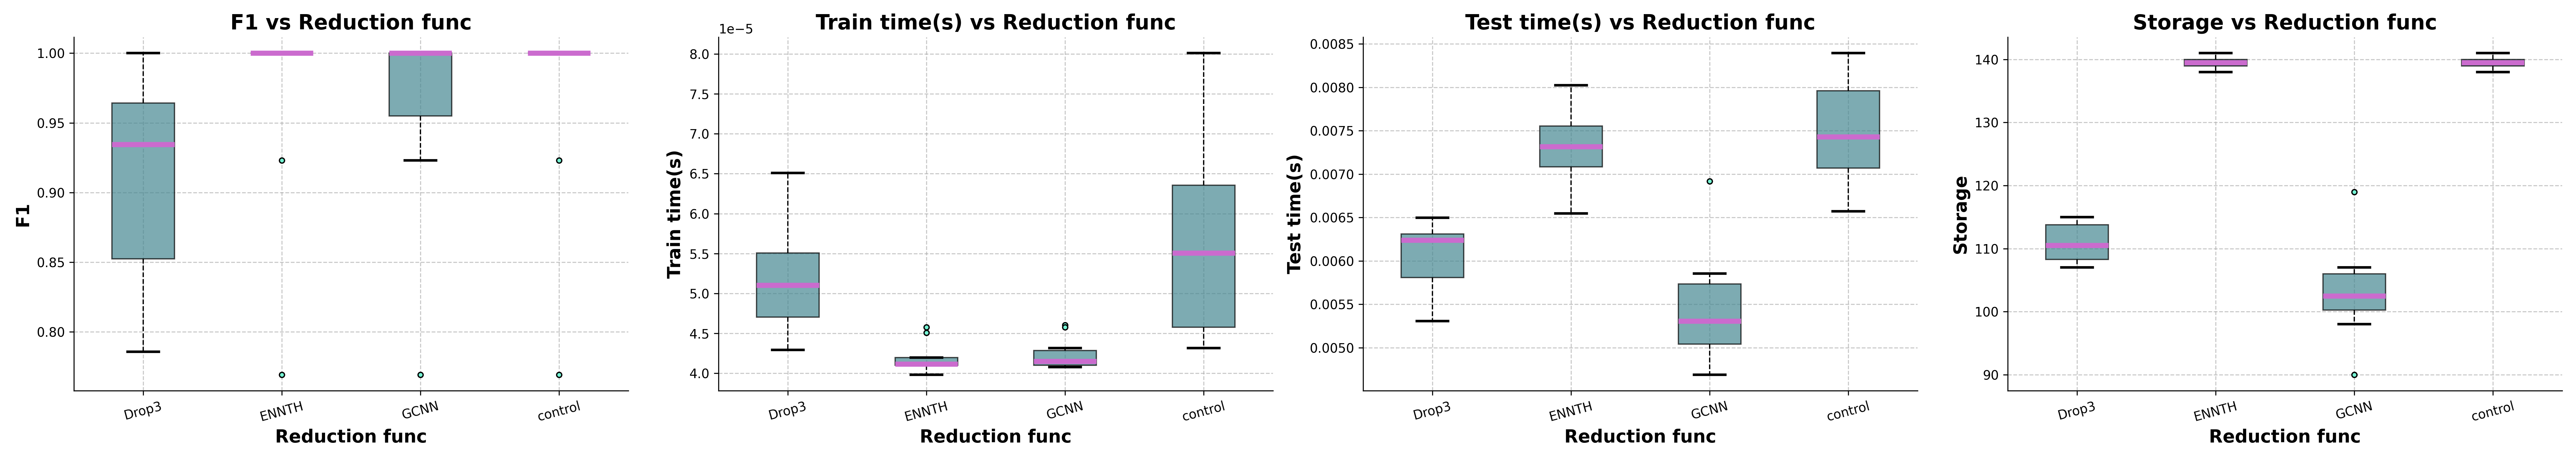
\includegraphics[width=0.45\textwidth]{figures/work2/reports/figures/KNN_reduction_effects_hepatitis.png}
    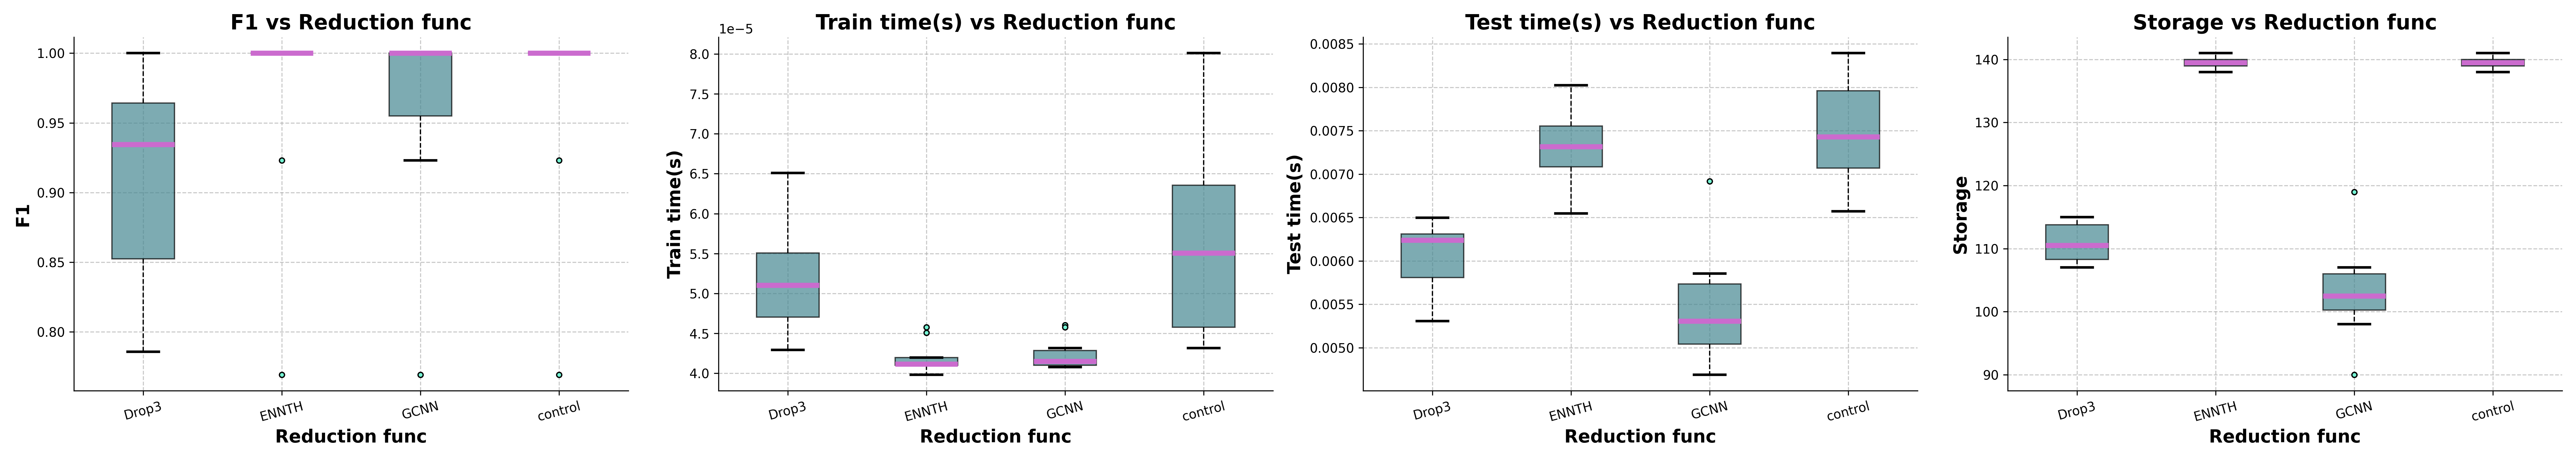
\includegraphics[width=0.45\textwidth]{figures/work2/reports/figures/KNN_reduction_effects_hepatitis.png}
    \caption{Class distributions}
    \label{fig:class-distributions}
\end{figure}

Overall, GGCN emerges as the most effective reduction technique across both models, showcasing substantial efficiency gains while preserving predictive accuracy, particularly for larger datasets like Mushroom.



\subsubsection{Support Vector Machines (SVM) Analysis}
\label{subsubsec:discussion-svm}

This section interprets the results of the SVM algorithm, discussing its performance and implications.

% TODO: Summarize the performance metrics of SVM (e.g., accuracy, precision, recall)
% TODO: Compare SVM results with other methods used in the study
% TODO: Discuss the impact of different kernel functions and hyperparameters
% TODO: Address any unexpected findings or limitations specific to SVM

% Add more content here as needed


% Add more content here as needed


\section{Conclusion}
\label{sec:conclusion}

This study has provided a comprehensive evaluation of KNN and SVM classification algorithms, along with instance reduction techniques, across two distinctly different datasets. Our analysis yields several important findings and practical implications.

\subsection{Key Findings}

\begin{itemize}
    \item Both KNN and SVM achieved high classification accuracy (\textgreater 92\%) across both datasets, demonstrating their robustness as classification algorithms
    \item The optimal configuration for KNN varied significantly between datasets, with k=1 performing best for Hepatitis and k=3,5,7 for Mushroom
    \item Instance reduction techniques, particularly GCNN, successfully reduced storage requirements while maintaining classification accuracy
    \item Statistical analysis revealed significant differences between model configurations, highlighting the importance of parameter tuning
    \item The top-performing models tended to have very similar F1 scores, suggesting there isn't a single perfect model for all datasets
    \item SVM configurations with higher C values tended to perform better, suggesting that greater regularization is better for both datasets.
\end{itemize}

\subsection{Practical Implications}

Our results suggest several practical guidelines for practitioners:
\begin{itemize}
    \item For smaller datasets with mixed data types (like Hepatitis), both RBF and polynomial kernels in SVM provide excellent performance
    \item For larger categorical datasets (like Mushroom), SVM with either polynomial or RBF kernels and higher C values (C=5 or C=50) achieves optimal results
    \item GCNN reduction can significantly improve efficiency without substantial accuracy loss, especially for larger datasets
    \item SVM with RBF kernel provides consistent performance across different dataset characteristics
\end{itemize}

\subsection{Limitations and Future Work}

While this study provides valuable insights, several limitations and opportunities for future research remain:
\begin{itemize}
    \item Investigation of additional datasets with different characteristics would strengthen the generalizability of our findings
    \item Exploration of more sophisticated reduction techniques could potentially yield better efficiency-accuracy trade-offs
    \item Analysis of computational complexity and memory usage could provide deeper insights into algorithm scalability
\end{itemize}

\subsection{Final Remarks}

This study demonstrates that both KNN and SVM remain powerful classification algorithms when properly configured. The effectiveness of instance reduction techniques, particularly GCNN, suggests that these methods can significantly improve the practical applicability of instance-based learning. These findings contribute to the ongoing development of efficient and accurate classification systems in machine learning.


\bibliography{references}
\newpage
\section{Appendix}
\label{sec:appendix}
\begin{longtable}{c|c|c|c|c}
\caption{KNN Legend} \label{tab:KNN_legend} \\
\hline
Model Label & K & Distance Func & Voting Func & Weighting Func \\
\hline
\endfirsthead

\multicolumn{5}{c}{ KNN Legend -- Continued} \\
\hline
Model Label & K & Distance Func & Voting Func & Weighting Func \\
\hline
\endhead

\hline
\multicolumn{5}{r}{Continued on next page}
\endfoot

\hline
\endlastfoot
k1ChebShpEq & 1 & ChebyshevDistance & ShepardsWorkVote & EqualWeighting \\
k1ChebDisEq & 1 & ChebyshevDistance & InverseDistanceWeightedVote & EqualWeighting \\
k1ChebMajEq & 1 & ChebyshevDistance & MajorityClassVote & EqualWeighting \\
k5EucShpEq & 5 & EuclideanDistance & ShepardsWorkVote & EqualWeighting \\
k7EucShpEq & 7 & EuclideanDistance & ShepardsWorkVote & EqualWeighting \\
k3ManShpEq & 3 & ManhattanDistance & ShepardsWorkVote & EqualWeighting \\
k1EucShpRlf & 1 & EuclideanDistance & ShepardsWorkVote & ReliefFWeighting \\
k7ManShpEq & 7 & ManhattanDistance & ShepardsWorkVote & EqualWeighting \\
k1EucShpEq & 1 & EuclideanDistance & ShepardsWorkVote & EqualWeighting \\
k1EucDisRlf & 1 & EuclideanDistance & InverseDistanceWeightedVote & ReliefFWeighting \\
k1EucDisEq & 1 & EuclideanDistance & InverseDistanceWeightedVote & EqualWeighting \\
k1ManMajEq & 1 & ManhattanDistance & MajorityClassVote & EqualWeighting \\
k5ManShpEq & 5 & ManhattanDistance & ShepardsWorkVote & EqualWeighting \\
k1EucMajEq & 1 & EuclideanDistance & MajorityClassVote & EqualWeighting \\
k1ManShpEq & 1 & ManhattanDistance & ShepardsWorkVote & EqualWeighting \\
k1ManDisEq & 1 & ManhattanDistance & InverseDistanceWeightedVote & EqualWeighting \\
k1EucMajRlf & 1 & EuclideanDistance & MajorityClassVote & ReliefFWeighting \\
k7ManShpRlf & 7 & ManhattanDistance & ShepardsWorkVote & ReliefFWeighting \\
k1ManShpRlf & 1 & ManhattanDistance & ShepardsWorkVote & ReliefFWeighting \\
k1ManDisRlf & 1 & ManhattanDistance & InverseDistanceWeightedVote & ReliefFWeighting \\
k3ManShpRlf & 3 & ManhattanDistance & ShepardsWorkVote & ReliefFWeighting \\
k5ManShpRlf & 5 & ManhattanDistance & ShepardsWorkVote & ReliefFWeighting \\
k1ManMajRlf & 1 & ManhattanDistance & MajorityClassVote & ReliefFWeighting \\
k3EucShpRlf & 3 & EuclideanDistance & ShepardsWorkVote & ReliefFWeighting \\
k3EucShpEq & 3 & EuclideanDistance & ShepardsWorkVote & EqualWeighting \\
k3ManDisEq & 3 & ManhattanDistance & InverseDistanceWeightedVote & EqualWeighting \\
k5ChebShpEq & 5 & ChebyshevDistance & ShepardsWorkVote & EqualWeighting \\
k7EucShpRlf & 7 & EuclideanDistance & ShepardsWorkVote & ReliefFWeighting \\
k5EucShpRlf & 5 & EuclideanDistance & ShepardsWorkVote & ReliefFWeighting \\
k5ChebDisEq & 5 & ChebyshevDistance & InverseDistanceWeightedVote & EqualWeighting \\
k3EucDisEq & 3 & EuclideanDistance & InverseDistanceWeightedVote & EqualWeighting \\
k3ChebShpEq & 3 & ChebyshevDistance & ShepardsWorkVote & EqualWeighting \\
k5ManDisEq & 5 & ManhattanDistance & InverseDistanceWeightedVote & EqualWeighting \\
k3ChebDisEq & 3 & ChebyshevDistance & InverseDistanceWeightedVote & EqualWeighting \\
k1ChebDisRlf & 1 & ChebyshevDistance & InverseDistanceWeightedVote & ReliefFWeighting \\
k1ChebShpRlf & 1 & ChebyshevDistance & ShepardsWorkVote & ReliefFWeighting \\
k1ChebMajRlf & 1 & ChebyshevDistance & MajorityClassVote & ReliefFWeighting \\
k5EucDisEq & 5 & EuclideanDistance & InverseDistanceWeightedVote & EqualWeighting \\
k7ManDisEq & 7 & ManhattanDistance & InverseDistanceWeightedVote & EqualWeighting \\
k5ChebMajEq & 5 & ChebyshevDistance & MajorityClassVote & EqualWeighting \\
k7EucDisEq & 7 & EuclideanDistance & InverseDistanceWeightedVote & EqualWeighting \\
k7ChebShpRlf & 7 & ChebyshevDistance & ShepardsWorkVote & ReliefFWeighting \\
k7ChebDisEq & 7 & ChebyshevDistance & InverseDistanceWeightedVote & EqualWeighting \\
k7ChebShpEq & 7 & ChebyshevDistance & ShepardsWorkVote & EqualWeighting \\
k5ChebShpRlf & 5 & ChebyshevDistance & ShepardsWorkVote & ReliefFWeighting \\
k3ChebShpRlf & 3 & ChebyshevDistance & ShepardsWorkVote & ReliefFWeighting \\
k3EucDisRlf & 3 & EuclideanDistance & InverseDistanceWeightedVote & ReliefFWeighting \\
k3EucMajRlf & 3 & EuclideanDistance & MajorityClassVote & ReliefFWeighting \\
k5EucDisRlf & 5 & EuclideanDistance & InverseDistanceWeightedVote & ReliefFWeighting \\
k5EucMajRlf & 5 & EuclideanDistance & MajorityClassVote & ReliefFWeighting \\
k5ChebDisRlf & 5 & ChebyshevDistance & InverseDistanceWeightedVote & ReliefFWeighting \\
k3ChebDisRlf & 3 & ChebyshevDistance & InverseDistanceWeightedVote & ReliefFWeighting \\
k7EucDisRlf & 7 & EuclideanDistance & InverseDistanceWeightedVote & ReliefFWeighting \\
k7EucMajRlf & 7 & EuclideanDistance & MajorityClassVote & ReliefFWeighting \\
k5EucMajEq & 5 & EuclideanDistance & MajorityClassVote & EqualWeighting \\
k5ManMajEq & 5 & ManhattanDistance & MajorityClassVote & EqualWeighting \\
k3ChebMajRlf & 3 & ChebyshevDistance & MajorityClassVote & ReliefFWeighting \\
k7ChebDisRlf & 7 & ChebyshevDistance & InverseDistanceWeightedVote & ReliefFWeighting \\
k7ManDisRlf & 7 & ManhattanDistance & InverseDistanceWeightedVote & ReliefFWeighting \\
k7ManMajRlf & 7 & ManhattanDistance & MajorityClassVote & ReliefFWeighting \\
k3ManMajRlf & 3 & ManhattanDistance & MajorityClassVote & ReliefFWeighting \\
k3ManDisRlf & 3 & ManhattanDistance & InverseDistanceWeightedVote & ReliefFWeighting \\
k5ChebMajRlf & 5 & ChebyshevDistance & MajorityClassVote & ReliefFWeighting \\
k5ManMajRlf & 5 & ManhattanDistance & MajorityClassVote & ReliefFWeighting \\
k5ManDisRlf & 5 & ManhattanDistance & InverseDistanceWeightedVote & ReliefFWeighting \\
k3EucMajEq & 3 & EuclideanDistance & MajorityClassVote & EqualWeighting \\
k3ManMajEq & 3 & ManhattanDistance & MajorityClassVote & EqualWeighting \\
k7EucMajEq & 7 & EuclideanDistance & MajorityClassVote & EqualWeighting \\
k7ManMajEq & 7 & ManhattanDistance & MajorityClassVote & EqualWeighting \\
k7ChebMajRlf & 7 & ChebyshevDistance & MajorityClassVote & ReliefFWeighting \\
k3ChebMajEq & 3 & ChebyshevDistance & MajorityClassVote & EqualWeighting \\
k1EucMajInf & 1 & EuclideanDistance & MajorityClassVote & InformationGainWeighting \\
k1EucDisInf & 1 & EuclideanDistance & InverseDistanceWeightedVote & InformationGainWeighting \\
k7EucMajInf & 7 & EuclideanDistance & MajorityClassVote & InformationGainWeighting \\
k7ManShpInf & 7 & ManhattanDistance & ShepardsWorkVote & InformationGainWeighting \\
k1ManShpInf & 1 & ManhattanDistance & ShepardsWorkVote & InformationGainWeighting \\
k7EucDisInf & 7 & EuclideanDistance & InverseDistanceWeightedVote & InformationGainWeighting \\
k3ChebMajInf & 3 & ChebyshevDistance & MajorityClassVote & InformationGainWeighting \\
k7EucShpInf & 7 & EuclideanDistance & ShepardsWorkVote & InformationGainWeighting \\
k1ManDisInf & 1 & ManhattanDistance & InverseDistanceWeightedVote & InformationGainWeighting \\
k7ChebMajEq & 7 & ChebyshevDistance & MajorityClassVote & EqualWeighting \\
k7ChebMajInf & 7 & ChebyshevDistance & MajorityClassVote & InformationGainWeighting \\
k7ChebDisInf & 7 & ChebyshevDistance & InverseDistanceWeightedVote & InformationGainWeighting \\
k3EucDisInf & 3 & EuclideanDistance & InverseDistanceWeightedVote & InformationGainWeighting \\
k7ChebShpInf & 7 & ChebyshevDistance & ShepardsWorkVote & InformationGainWeighting \\
k1EucShpInf & 1 & EuclideanDistance & ShepardsWorkVote & InformationGainWeighting \\
k7ManMajInf & 7 & ManhattanDistance & MajorityClassVote & InformationGainWeighting \\
k7ManDisInf & 7 & ManhattanDistance & InverseDistanceWeightedVote & InformationGainWeighting \\
k3ChebShpInf & 3 & ChebyshevDistance & ShepardsWorkVote & InformationGainWeighting \\
k5ManDisInf & 5 & ManhattanDistance & InverseDistanceWeightedVote & InformationGainWeighting \\
k3ManShpInf & 3 & ManhattanDistance & ShepardsWorkVote & InformationGainWeighting \\
k5ManShpInf & 5 & ManhattanDistance & ShepardsWorkVote & InformationGainWeighting \\
k5ManMajInf & 5 & ManhattanDistance & MajorityClassVote & InformationGainWeighting \\
k5EucMajInf & 5 & EuclideanDistance & MajorityClassVote & InformationGainWeighting \\
k1ManMajInf & 1 & ManhattanDistance & MajorityClassVote & InformationGainWeighting \\
k3ManDisInf & 3 & ManhattanDistance & InverseDistanceWeightedVote & InformationGainWeighting \\
k5EucDisInf & 5 & EuclideanDistance & InverseDistanceWeightedVote & InformationGainWeighting \\
k5EucShpInf & 5 & EuclideanDistance & ShepardsWorkVote & InformationGainWeighting \\
k3ManMajInf & 3 & ManhattanDistance & MajorityClassVote & InformationGainWeighting \\
k5ChebMajInf & 5 & ChebyshevDistance & MajorityClassVote & InformationGainWeighting \\
k3EucShpInf & 3 & EuclideanDistance & ShepardsWorkVote & InformationGainWeighting \\
k5ChebDisInf & 5 & ChebyshevDistance & InverseDistanceWeightedVote & InformationGainWeighting \\
k3EucMajInf & 3 & EuclideanDistance & MajorityClassVote & InformationGainWeighting \\
k5ChebShpInf & 5 & ChebyshevDistance & ShepardsWorkVote & InformationGainWeighting \\
k3ChebDisInf & 3 & ChebyshevDistance & InverseDistanceWeightedVote & InformationGainWeighting \\
k1ChebMajInf & 1 & ChebyshevDistance & MajorityClassVote & InformationGainWeighting \\
k1ChebDisInf & 1 & ChebyshevDistance & InverseDistanceWeightedVote & InformationGainWeighting \\
k1ChebShpInf & 1 & ChebyshevDistance & ShepardsWorkVote & InformationGainWeighting \\
\end{longtable}
\begin{table}
\centering
\caption{KNN-Reduction Legend}
\label{tab:KNN-Reduction_legend}
\begin{tabular}{lrlll}
\toprule
Model Label & K & Distance Func & Voting Func & Weighting Func \\
\midrule
Ctrlk1ManMajEq & 1 & ManhattanDistance & MajorityClassVote & EqualWeighting \\
Ennthk1ManMajEq & 1 & ManhattanDistance & MajorityClassVote & EqualWeighting \\
Ggcnk1ManMajEq & 1 & ManhattanDistance & MajorityClassVote & EqualWeighting \\
Drop3k1ManMajEq & 1 & ManhattanDistance & MajorityClassVote & EqualWeighting \\
\bottomrule
\end{tabular}
\end{table}

\begin{table}
\centering
\caption{SVM Legend}
\label{tab:SVM_legend}
\begin{tabular}{lrl}
\toprule
Model Label & C & Kernel Type \\
\midrule
C0.05Lin & 0.050 & linear \\
C0.05Poly & 0.050 & poly \\
C0.05Rbf & 0.050 & rbf \\
C0.05Sig & 0.050 & sigmoid \\
C0.5Lin & 0.500 & linear \\
C0.5Poly & 0.500 & poly \\
C0.5Rbf & 0.500 & rbf \\
C0.5Sig & 0.500 & sigmoid \\
C5Lin & 5.000 & linear \\
C5Poly & 5.000 & poly \\
C5Rbf & 5.000 & rbf \\
C5Sig & 5.000 & sigmoid \\
C50Lin & 50.000 & linear \\
C50Poly & 50.000 & poly \\
C50Rbf & 50.000 & rbf \\
C50Sig & 50.000 & sigmoid \\
\bottomrule
\end{tabular}
\end{table}

\begin{table}
\centering
\caption{SVM-Reduction Legend}
\label{tab:SVM-Reduction_legend}
\begin{tabular}{lrl}
\toprule
Model Label & C & Kernel Type \\
\midrule
CtrlC7Rbf & 7 & rbf \\
GcnnC7Rbf & 7 & rbf \\
EnnthC7Rbf & 7 & rbf \\
Drop3C7Rbf & 7 & rbf \\
\bottomrule
\end{tabular}
\end{table}

\end{document}
